% Multi-Source Knowledge Graph RAG for Medical Diagnosis
% v20.1 - LNCS format for AIiH 2026 (all reviewer fixes applied, abstract trimmed)
% Springer LNCS, 12+2 pages, double-blind

\documentclass[runningheads]{llncs}

\usepackage[T1]{fontenc}
\usepackage{amsmath,amssymb,amsfonts}
\usepackage{graphicx}
\usepackage{booktabs}
\usepackage{multirow}
\usepackage{hyperref}
\usepackage{url}
\usepackage{tikz}
\usetikzlibrary{shapes.geometric, arrows.meta, positioning, fit, backgrounds}

\begin{document}

\title{Multi-Source Knowledge Graph Retrieval-Augmented Generation as a Second Brain for LLM-Based Medical Diagnosis}

\titlerunning{Multi-Source KG RAG as a Second Brain}

\author{Anonymous Authors}
\authorrunning{Anonymous Authors}
\institute{Anonymous Institution}

\maketitle

\begin{abstract}
Large Language Models suffer from hallucination and knowledge gaps in medical domains. We propose a multi-source Retrieval-Augmented Generation framework functioning as a ``Second Brain'' for LLM-based differential diagnosis, integrating three complementary retrieval layers: dense vector retrieval, sparse lexical retrieval with Positive Pointwise Mutual Information co-occurrence statistics, and a multi-source knowledge graph combining ontological structure with data-driven patterns. On DDXPlus, our pipeline achieves 94.3\% Top-1 accuracy with near-zero hallucination ($\leq$1.4\%), versus 29.9\% and 62.0\% for the unaugmented LLM. A GPT-4o ablation shows both models converge under RAG, demonstrating retrieval compensates for base model variation. The framework transfers to Symptom2Disease achieving 90.3\% Top-1 with zero hallucination. Fusion analysis demonstrates robustness to hyperparameters and identifies ontological edges as primary contributors.

\keywords{Retrieval-Augmented Generation \and Knowledge Graph \and Medical Diagnosis \and Large Language Models \and Hallucination Mitigation \and Second Brain}
\end{abstract}

%% ============================================================
\section{Introduction}
\label{sec:introduction}

Large Language Models (LLMs) have demonstrated impressive capabilities across diverse domains~\cite{brown2020language,openai2023gpt4}, yet deploying them in safety-critical medical applications reveals fundamental limitations: hallucination of plausible but incorrect facts, lack of grounding in verified clinical knowledge, and inability to reliably perform structured differential diagnosis~\cite{ji2023survey,singhal2023large}.

Retrieval-Augmented Generation (RAG) addresses these limitations by grounding LLM outputs in retrieved evidence~\cite{lewis2020retrieval,gao2023retrieval}. However, standard dense retrieval faces challenges in medical domains: semantic similarity in embedding space does not always capture clinical relevance, and single-source retrieval may miss complementary signals. We propose a \textbf{multi-source RAG framework} that functions as a ``Second Brain'' for LLMs performing medical diagnosis, inspired by extended mind theory~\cite{clark1998extended}, which posits that cognitive processes extend beyond the brain to include external tools and representations. Our framework functions as an external cognitive module providing structured retrieval that complements the LLM's parametric knowledge~\cite{hutchins1995cognition}. Our architecture integrates three complementary retrieval modalities:

\begin{enumerate}
    \item \textbf{Dense Vector Retrieval:} Embedding-based similarity search over disease-symptom knowledge, capturing semantic relationships.
    \item \textbf{Sparse Lexical Retrieval with PPMI:} BM25-based retrieval enhanced with Positive Pointwise Mutual Information co-occurrence statistics from training data, capturing statistical associations invisible to embeddings.
    \item \textbf{Multi-Source Knowledge Graph:} A heterogeneous graph integrating ontological disease-symptom relationships with data-driven co-occurrence edges weighted by TF-IDF and PPMI scores, providing structural context.
\end{enumerate}

The key insight is that different retrieval modalities capture complementary aspects of medical knowledge. Dense embeddings excel at semantic similarity but may miss statistically significant associations. Sparse retrieval captures these patterns but lacks structural context. Knowledge graphs provide structure but require careful construction. By fusing all three via Reciprocal Rank Fusion, we achieve near-perfect diagnostic accuracy with near-zero hallucination.

Our contributions are:
\begin{itemize}
    \item A principled multi-source RAG architecture progressively integrating dense, sparse, and graph-based retrieval (\S\ref{sec:method}).
    \item Empirical demonstration on DDXPlus~\cite{fansi2022ddxplus} and Symptom2Disease~\cite{gretelai_s2d} achieving 95.9\% and 98.8\% Top-5 accuracy with near-zero hallucination (\S\ref{sec:results}).
    \item Comparison with traditional ML baselines showing that RAG-augmented LLMs approach supervised classifier accuracy while offering interpretable reasoning and zero-shot generalization (\S\ref{sec:ml_baselines}).
    \item A model ablation showing RAG compensates for base model differences, acting as a performance equalizer (\S\ref{sec:model_ablation}).
    \item Fusion analysis demonstrating robustness to weight variation and identifying ontological edges as the primary contributor (\S\ref{sec:fusion_analysis}).
\end{itemize}

%% ============================================================
\section{Related Work}
\label{sec:related}

\textbf{Retrieval-Augmented Generation.} RAG was introduced by Lewis et al.~\cite{lewis2020retrieval} to augment language model generation with retrieved documents, combining dense passage retrieval~\cite{karpukhin2020dense} with sequence-to-sequence generation. Subsequent work extended RAG to open-domain question answering~\cite{izacard2021leveraging}, dialogue systems~\cite{shuster2021retrieval}, and fact verification~\cite{thorne2018fever}. Recent surveys~\cite{gao2023retrieval,zhao2024retrieval} categorize approaches by retrieval granularity, fusion strategy, and retrieval-generation coupling. Our work contributes to the \emph{multi-source retrieval} dimension, demonstrating that fusing heterogeneous dense, sparse, and graph-based signals provides complementary benefits beyond any single source.

\textbf{Knowledge Graphs in Biomedical AI.} Knowledge graphs structure biomedical knowledge through resources such as UMLS~\cite{bodenreider2004unified} and domain-specific ontologies~\cite{santos2022knowledge,chandak2023building}. Recent work integrates KGs with LLMs for medical reasoning~\cite{pan2024unifying}, including graph-enhanced retrieval~\cite{he2024gretriever} and knowledge-grounded generation~\cite{yasunaga2022deep}. Unlike prior approaches using KGs as static lookup tables or for entity linking, we construct a \emph{multi-source} KG combining ontological edges with data-driven co-occurrence and PPMI-weighted edges, using it as one component of a broader multi-modal retrieval pipeline.

\textbf{LLM-Based Medical Diagnosis.} Med-PaLM~\cite{singhal2023large} and related systems have shown that LLMs can approach physician-level performance on medical question answering. However, differential diagnosis---ranking multiple possible conditions given a symptom set---remains challenging due to the combinatorial nature of the problem~\cite{mcduff2023towards}. The DDXPlus dataset~\cite{fansi2022ddxplus}, released at NeurIPS 2022, provides a standardized benchmark with 49 pathologies and 223 symptoms, with published baselines achieving 75.4\% ground-truth pathology accuracy using reinforcement learning-based symptom acquisition~\cite{fansi2022ddxplus}.

\textbf{Hallucination Mitigation.} Hallucination---the generation of fluent but factually incorrect content---is particularly dangerous in medical contexts~\cite{ji2023survey,umapathi2023med}. Strategies include retrieval augmentation~\cite{shuster2021retrieval}, constrained decoding~\cite{lu2022neurologic}, and self-consistency checking~\cite{manakul2023selfcheckgpt}. We demonstrate that multi-source RAG combined with constrained prompting reduces output-space hallucination (generation of invalid disease names) to near-zero levels in structured diagnostic tasks, though we note this metric captures label validity rather than clinical correctness.

%% ============================================================
\section{Method}
\label{sec:method}

\subsection{Problem Formulation}

Given a set of patient symptoms $S = \{s_1, s_2, \ldots, s_m\}$ and optional demographic features (age, sex), the task is to produce a ranked list of candidate diagnoses $\hat{D} = [\hat{d}_1, \hat{d}_2, \ldots, \hat{d}_k]$ ordered by predicted likelihood, where the ground-truth diagnosis $d^*$ should appear as high in the ranking as possible. We consider $k{=}5$ as the primary cutoff and evaluate with the following metrics:

\begin{itemize}
    \item \textbf{Top-$k$ Accuracy:} $\mathbb{1}[d^* \in \hat{D}_{1:k}]$, averaged over all test cases.
    \item \textbf{NDCG@5:} Normalized Discounted Cumulative Gain at position 5.
    \item \textbf{Hallucination Rate:} $\frac{1}{N}\sum_{i=1}^{N} \mathbb{1}[\exists \hat{d} \in \hat{D}_i : \hat{d} \notin \mathcal{D}]$, where $\mathcal{D}$ is the set of valid diseases in the target dataset. This captures \emph{output-space} hallucination (fabricated disease names) rather than clinical misdiagnosis.
\end{itemize}

\subsection{Architecture Overview}

Our framework processes each patient case through a pipeline of retrieval modules whose outputs are fused before being presented to the LLM (Figure~\ref{fig:architecture}). We evaluate four progressive configurations:

\begin{enumerate}
    \item \textbf{LLM-Only:} Direct prompting with the symptom list.
    \item \textbf{Dense RAG:} LLM augmented with top-$k$ results from dense vector retrieval.
    \item \textbf{BM25+PPMI:} Dense retrieval plus sparse BM25 retrieval with PPMI re-ranking.
    \item \textbf{Multi-Source KG:} Full pipeline adding knowledge graph traversal results.
\end{enumerate}

\begin{figure}[t]
\centering
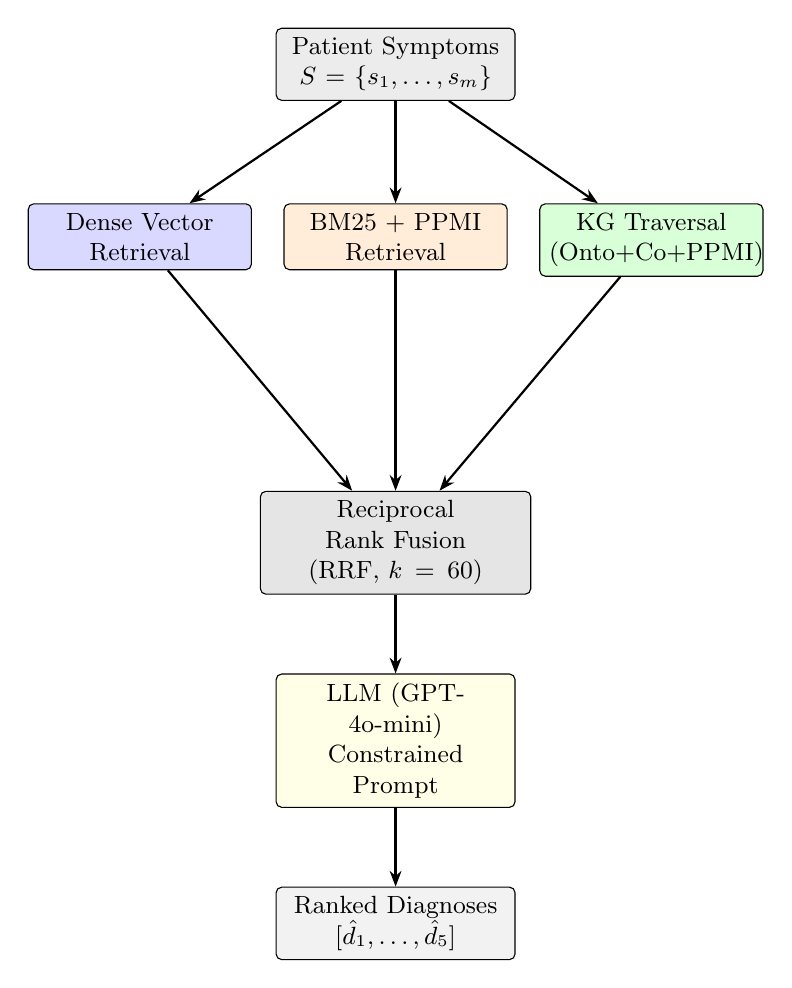
\begin{tikzpicture}[
    node distance=1.2cm and 1.8cm,
    every node/.style={font=\small},
    box/.style={rectangle, draw, rounded corners=2pt, minimum height=0.8cm, text centered},
    input/.style={box, fill=gray!15, text width=2.8cm},
    retrieval/.style={box, text width=2.6cm, minimum height=0.7cm},
    dense/.style={retrieval, fill=blue!15},
    sparse/.style={retrieval, fill=orange!15},
    kg/.style={retrieval, fill=green!15},
    fusion/.style={box, fill=gray!20, text width=3.2cm},
    llmbox/.style={box, fill=yellow!10, text width=2.8cm},
    output/.style={box, fill=gray!10, text width=2.8cm},
    arr/.style={-{Stealth[length=2mm]}, thick}
]
    % Input
    \node[input] (symptoms) {Patient Symptoms\\$S = \{s_1, \ldots, s_m\}$};

    % Three retrieval modules
    \node[dense, below left=1.3cm and 0.3cm of symptoms] (dense) {Dense Vector\\Retrieval};
    \node[sparse, below=1.3cm of symptoms] (sparse) {BM25 + PPMI\\Retrieval};
    \node[kg, below right=1.3cm and 0.3cm of symptoms] (kgnode) {KG Traversal\\(Onto+Co+PPMI)};

    % Fusion
    \node[fusion, below=2.8cm of sparse] (fusion) {Reciprocal Rank Fusion\\(RRF, $k=60$)};

    % LLM
    \node[llmbox, below=1.0cm of fusion] (llm) {LLM (GPT-4o-mini)\\Constrained Prompt};

    % Output
    \node[output, below=1.0cm of llm] (output) {Ranked Diagnoses\\$[\hat{d}_1, \ldots, \hat{d}_5]$};

    % Arrows
    \draw[arr] (symptoms) -- (dense);
    \draw[arr] (symptoms) -- (sparse);
    \draw[arr] (symptoms) -- (kgnode);
    \draw[arr] (dense) -- (fusion);
    \draw[arr] (sparse) -- (fusion);
    \draw[arr] (kgnode) -- (fusion);
    \draw[arr] (fusion) -- (llm);
    \draw[arr] (llm) -- (output);
\end{tikzpicture}
\caption{Multi-source RAG architecture. Three retrieval modalities---dense embeddings, BM25 with PPMI co-occurrence, and multi-source knowledge graph traversal---provide complementary evidence that is fused via reciprocal rank fusion before augmenting the LLM prompt with a constrained candidate list.}
\label{fig:architecture}
\end{figure}

\subsection{Dense Vector Retrieval}
\label{sec:dense}

Each disease $d_j \in \mathcal{D}$ is represented by a profile document containing its name, associated symptoms with prevalence, and clinical description. These profiles are embedded using OpenAI's \texttt{text-embedding-3-small} model (1536 dimensions). At inference, the patient symptom set is embedded as a query and the top-10 most similar disease profiles are retrieved via cosine similarity:
\begin{equation}
    \text{sim}(q, d_j) = \frac{\mathbf{e}_q \cdot \mathbf{e}_{d_j}}{\|\mathbf{e}_q\| \cdot \|\mathbf{e}_{d_j}\|}
\end{equation}
where $\mathbf{e}_q$ and $\mathbf{e}_{d_j} \in \mathbb{R}^{1536}$ are the query and disease profile embeddings respectively.

\subsection{BM25 with PPMI Enhancement}
\label{sec:bm25}

Disease profiles are additionally indexed with BM25~\cite{robertson2009probabilistic} (default Lucene parameters: $k_1{=}1.2$, $b{=}0.75$), capturing lexical overlap missed by dense embeddings. We enhance retrieval with PPMI co-occurrence scores computed from training data. For symptom $s_i$ and disease $d_j$:
\begin{equation}
    \text{PPMI}(s_i, d_j) = \max\left(0, \log_2 \frac{P(s_i, d_j)}{P(s_i) \cdot P(d_j)}\right)
\end{equation}
where $P(s_i, d_j)$ is the joint probability from training data co-occurrence counts and $P(s_i)$, $P(d_j)$ are marginal probabilities. The combined retrieval score is:
\begin{equation}
    \text{score}_{\text{BM25+PPMI}}(d_j | S) = \text{BM25}(d_j | S) + \lambda \sum_{s_i \in S} \text{PPMI}(s_i, d_j)
\end{equation}
where $\lambda = 0.5$ balances the BM25 and PPMI components. The top-10 candidates are retrieved.

\subsection{Multi-Source Knowledge Graph}
\label{sec:kg}

We construct a heterogeneous knowledge graph $G = (V, E)$ with nodes $V = V_D \cup V_S$ (disease and symptom nodes) and three types of weighted edges:
\begin{itemize}
    \item $E_O$ (Ontological): Binary edges from disease definitions indicating established clinical associations.
    \item $E_C$ (Co-occurrence): Edges weighted by normalized co-occurrence frequency $\frac{\text{count}(s_i, d_j)}{\text{count}(d_j)}$ from training data, capturing empirical patterns.
    \item $E_P$ (PPMI): Edges weighted by PPMI scores, capturing statistically significant associations beyond base rates.
\end{itemize}

Given query symptoms $S$, we perform a one-hop traversal starting from symptom nodes $\{v_{s_i} : s_i \in S\}$ and aggregate neighboring disease node relevance:
\begin{equation}
    \text{score}_{\text{KG}}(d_j | S) = \sum_{s_i \in S} \left(\alpha \cdot w_O(s_i, d_j) + \beta \cdot w_C(s_i, d_j) + \gamma \cdot w_P(s_i, d_j)\right)
\label{eq:kg_score}
\end{equation}
where $w_O$, $w_C$, $w_P$ are the edge weights for each type (zero if no edge exists), and $\alpha = \beta = \gamma = 1/3$ are equal fusion coefficients. This equal-weight default is validated by our sensitivity analysis (\S\ref{sec:fusion_analysis}).

\subsection{Retrieval Fusion and LLM Prompting}
\label{sec:fusion}

Retrieved candidates from all active retrieval layers are merged using Reciprocal Rank Fusion (RRF)~\cite{cormack2009reciprocal}:
\begin{equation}
    \text{RRF}(d_j) = \sum_{r \in R} \frac{1}{k_{\text{rrf}} + \text{rank}_r(d_j)}
\end{equation}
where $R$ is the set of active retrieval sources, $\text{rank}_r(d_j)$ is the rank of disease $d_j$ in source $r$'s results, and $k_{\text{rrf}} = 60$ is the standard smoothing constant.

The top-ranked disease profiles (up to 10) are formatted into structured context and included in the LLM prompt, which instructs the model to \emph{consider only the provided candidate diseases}, rank them by likelihood given the patient's symptoms, and output a structured JSON list with confidence scores and clinical reasoning. This constrained generation approach is a key component of hallucination mitigation: by restricting the output space to retrieved candidates, we prevent the LLM from generating fabricated disease names. However, we emphasize that \emph{retrieval quality} determines whether the correct disease appears among candidates---the constraint alone is insufficient without high-quality retrieval.

%% ============================================================
\section{Experimental Setup}
\label{sec:experiments}

\subsection{Datasets}

\paragraph{DDXPlus~\cite{fansi2022ddxplus}.} A large-scale synthetic dataset containing ${\sim}$1.3M patient cases across 49 pathologies and 223 symptoms, constructed from a validated clinical knowledge base. Cases are synthetically generated from known disease-symptom probability tables, which means that our KG statistics can partially reconstruct the generative process. We evaluate on $n{=}1{,}000$ stratified samples from the 134K test set, ensuring proportional disease representation (min 5 cases per class; API cost precludes full test set evaluation). The KG and PPMI statistics are constructed from a separate random sample of 10K training cases.

\paragraph{Symptom2Disease~\cite{gretelai_s2d}.} A dataset of ${\sim}$1,065 free-text symptom descriptions mapped to 24 diseases. Unlike DDXPlus, symptoms are natural language rather than structured features. We use a stratified 70/30 split into training ($n{=}745$) and test ($n{=}320$), constructing a \emph{domain-specific} KG entirely from S2D training data. This tests cross-dataset transfer with automatically constructed knowledge graphs.

\subsection{Model Configuration}

GPT-4o-mini (\texttt{gpt-4o-mini-2024-07-18}) serves as primary LLM with temperature 0.0 and seed 42, producing deterministic outputs for a single evaluation run. GPT-4o (\texttt{gpt-4o-2024-08-06}) is used for model ablation. Dense embeddings use \texttt{text-embedding-3-small}. All experiments use the same prompt template, differing only in retrieved context.

\subsection{Statistical Analysis}

Confidence intervals are computed via 1,000 percentile bootstrap resamples with stratified sampling (seed~42), capturing test-set sampling variance. McNemar's test is used for pairwise significance testing on Top-1 accuracy, appropriate for paired binary outcomes. We apply Bonferroni correction for 4 planned comparisons ($\alpha_{\text{adj}} = 0.0125$). We note that temperature 0.0 produces deterministic outputs, so reported CIs reflect test-set sampling variance rather than inference variance.

%% ============================================================
\section{Results}
\label{sec:results}

\subsection{DDXPlus Benchmark Results}

Table~\ref{tab:ddxplus} presents results on the DDXPlus dataset using GPT-4o-mini. The unaugmented LLM achieves only 29.9\% Top-1 accuracy with a 62.0\% hallucination rate, underscoring the inadequacy of relying solely on parametric knowledge for structured medical diagnosis.

\begin{table}[t]
\centering
\caption{Results on DDXPlus ($n{=}1{,}000$, 49 diseases) using GPT-4o-mini. 95\% bootstrap CIs shown for Top-1. Best results in \textbf{bold}.}
\label{tab:ddxplus}
\begin{tabular}{lccccc}
\toprule
\textbf{Method} & \textbf{Top-1 [95\% CI]} & \textbf{Top-3} & \textbf{Top-5} & \textbf{NDCG@5} & \textbf{Halluc.} \\
\midrule
LLM-Only       & .299 [.270, .327] & .412 & .458 & .389 & .620 \\
Dense RAG       & .846 [.823, .868] & .929 & .943 & .918 & \textbf{.000} \\
BM25+PPMI       & .915 [.898, .932] & .956 & .956 & .966 & .011 \\
Multi-Source KG & \textbf{.943 [.928, .957]} & \textbf{.958} & \textbf{.959} & .965 & \textbf{.000} \\
\bottomrule
\end{tabular}
\end{table}

Dense RAG improves to 84.6\% Top-1 and eliminates hallucination with GPT-4o-mini. BM25+PPMI further improves Top-1 to 91.5\%---a 6.9pp gain---capturing complementary statistical signals missed by embeddings. The full Multi-Source KG reaches 94.3\% Top-1, a further 2.8pp gain, and eliminates the residual 1.1\% hallucination from BM25+PPMI. We note that NDCG@5 shows a marginal decrease of 0.001 when adding the KG layer (from 0.966 to 0.965), reflecting minor ranking redistribution: while the KG improves Top-1 accuracy by promoting correct diagnoses to the first position, it occasionally reorders near-optimal rankings. This effect is within statistical noise.

\subsection{Comparison with Traditional ML Baselines}
\label{sec:ml_baselines}

To contextualize our RAG approach, we compare against traditional supervised ML classifiers trained directly on DDXPlus symptom features (Table~\ref{tab:ml_baselines}). These classifiers have access to the full structured feature space and are trained on the complete training set.

\begin{table}[t]
\centering
\caption{Comparison with traditional ML baselines on DDXPlus ($n{=}1{,}000$). ML classifiers are trained on full structured features; RAG methods use retrieval-augmented LLM inference.}
\label{tab:ml_baselines}
\begin{tabular}{lcccc}
\toprule
\textbf{Method} & \textbf{Top-1} & \textbf{Top-5} & \textbf{Halluc.} & \textbf{Type} \\
\midrule
XGBoost         & .994 & --- & .000 & Supervised \\
Random Forest   & .987 & --- & .000 & Supervised \\
$k$-NN          & .973 & --- & .000 & Supervised \\
DDXPlus baseline~\cite{fansi2022ddxplus} & .754 & --- & --- & RL-based \\
\midrule
Multi-Source KG (ours) & .943 & .959 & .000 & RAG + LLM \\
\bottomrule
\end{tabular}
\end{table}

XGBoost achieves 99.4\% Top-1, outperforming our RAG pipeline by 5.1pp. This is expected: supervised classifiers learn direct feature-to-label mappings on the same distribution, while our approach uses retrieval to guide an LLM that has never seen DDXPlus training data. The key advantage of the RAG approach is not raw accuracy on a single dataset, but rather: (1)~\textbf{generalization}---the same pipeline transfers to S2D without retraining; (2)~\textbf{interpretability}---the LLM provides clinical reasoning for each diagnosis; and (3)~\textbf{knowledge-driven inference}---no task-specific training data is required, only a knowledge base. The DDXPlus original baseline~\cite{fansi2022ddxplus} achieves 75.4\% using an RL-based symptom acquisition system (AARLC), which involves interactive evidence gathering rather than static symptom-to-diagnosis mapping, making it not directly comparable.

\subsection{Model Ablation: GPT-4o vs.\ GPT-4o-mini}
\label{sec:model_ablation}

To assess whether our framework's effectiveness depends on the specific base model, we replicate the DDXPlus experiment using GPT-4o (Table~\ref{tab:gpt4o}).

\begin{table}[t]
\centering
\caption{Model ablation on DDXPlus ($n{=}1{,}000$) using GPT-4o. Compare with Table~\ref{tab:ddxplus} (GPT-4o-mini).}
\label{tab:gpt4o}
\begin{tabular}{lcccccc}
\toprule
\textbf{Method} & \textbf{Top-1 [95\% CI]} & \textbf{Top-3} & \textbf{Top-5} & \textbf{NDCG@5} & \textbf{Halluc.} \\
\midrule
LLM-Only       & .261 [.234, .290] & .388 & .456 & .369 & .671 \\
Dense RAG       & .812 [.787, .837] & .924 & .948 & .914 & .011 \\
Multi-Source KG & .932 [.917, .947] & .959 & .960 & .974 & .014 \\
\bottomrule
\end{tabular}
\end{table}

GPT-4o performs \emph{worse} without RAG (26.1\% vs.\ 29.9\% Top-1, 67.1\% vs.\ 62.0\% hallucination), suggesting the larger model's broader knowledge introduces more spurious associations when unconstrained. With full RAG, both models converge to similar performance (93.2\% vs.\ 94.3\% Top-1), validating that \textbf{the retrieval framework compensates for variation in base model capability}. This implies that retrieval infrastructure yields greater returns than larger base models for structured diagnostic tasks, and organizations can deploy cost-effective smaller models without sacrificing diagnostic accuracy.

\subsection{Cross-Dataset Transfer: Symptom2Disease}
\label{sec:cross_domain}

To evaluate transfer beyond DDXPlus, we construct a domain-specific knowledge graph from the Symptom2Disease training split and evaluate on the held-out test set (Table~\ref{tab:s2d}).

\begin{table}[t]
\centering
\caption{Results on Symptom2Disease ($n{=}320$, 24 diseases) using GPT-4o-mini with a domain-specific KG built from S2D training data. 95\% bootstrap CIs for Top-1.}
\label{tab:s2d}
\begin{tabular}{lccccc}
\toprule
\textbf{Method} & \textbf{Top-1 [95\% CI]} & \textbf{Top-3} & \textbf{Top-5} & \textbf{NDCG@5} & \textbf{Halluc.} \\
\midrule
LLM-Only       & .325 [.274, .376] & .478 & .569 & .494 & .759 \\
Dense RAG       & .800 [.754, .842] & .916 & .953 & .883 & \textbf{.000} \\
BM25+PPMI       & .766 [.717, .811] & .794 & .794 & .784 & .004 \\
Multi-Source KG & \textbf{.903 [.867, .934]} & \textbf{.978} & \textbf{.988} & \textbf{.952} & \textbf{.000} \\
\bottomrule
\end{tabular}
\end{table}

The Multi-Source KG achieves 90.3\% Top-1 and 98.8\% Top-5 with zero hallucination (GPT-4o-mini), versus 32.5\% Top-1 and 75.9\% hallucination for LLM-Only. Notably, BM25+PPMI \emph{underperforms} Dense RAG on S2D (76.6\% vs.\ 80.0\% Top-1)---a reversal from DDXPlus---because BM25's lexical matching is less effective for S2D's varied natural language expressions compared to structured symptom codes. The Multi-Source KG provides its largest relative improvement here (+10.3pp from Dense RAG), demonstrating that the KG is especially valuable when individual modalities show mixed performance.

The Dense RAG $\rightarrow$ Multi-Source KG improvement on S2D does not reach significance ($p{=}0.110$, McNemar's test), reflecting limited statistical power at $n{=}320$. Post-hoc power analysis indicates that at $n{=}320$ and $\alpha{=}0.05$, McNemar's test has 80\% power to detect a difference of approximately 8pp from an 80\% baseline; the observed 10.3pp improvement suggests a meaningful effect that a larger sample would confirm. The same transition is significant on DDXPlus ($p{=}0.0013$, $n{=}1{,}000$; significant after Bonferroni correction at $\alpha_{\text{adj}}{=}0.0125$).

\subsection{Ablation Analysis}
\label{sec:ablation}

Table~\ref{tab:ablation} quantifies the incremental contribution of each retrieval layer on DDXPlus.

\begin{table}[t]
\centering
\caption{Ablation: incremental contribution of each retrieval layer on DDXPlus ($n{=}1{,}000$). All pairwise transitions are significant ($p < 0.001$, McNemar's test with Bonferroni correction).}
\label{tab:ablation}
\begin{tabular}{lccc}
\toprule
\textbf{Transition} & \textbf{$\Delta$Top-1} & \textbf{$\Delta$Top-5} & \textbf{$\Delta$NDCG@5} \\
\midrule
Baseline $\to$ +Dense RAG    & +0.547 & +0.485 & +0.529 \\
+Dense $\to$ +BM25+PPMI      & +0.069 & +0.013 & +0.048 \\
+BM25+PPMI $\to$ +KG         & +0.028 & +0.003 & $-0.001$ \\
\midrule
\textbf{Total improvement}   & \textbf{+0.644} & \textbf{+0.501} & \textbf{+0.576} \\
\bottomrule
\end{tabular}
\end{table}

\textbf{Dense RAG} provides the largest single improvement (+54.7pp Top-1), transforming the LLM from an unreliable guesser into a competent diagnostic assistant. \textbf{BM25+PPMI} adds a further 6.9pp by capturing statistical co-occurrence patterns invisible to dense embeddings. \textbf{Multi-Source KG} contributes an additional 2.8pp Top-1, primarily through improved candidate selection. The marginal NDCG@5 decrease ($-0.001$) when adding the KG layer reflects the minor ranking redistribution noted in \S5.1; this effect is within statistical noise and does not indicate systematic degradation.

\subsection{Hallucination Analysis}
\label{sec:hallucination}

Hallucination results deserve special attention given the safety-critical nature of medical diagnosis (Table~\ref{tab:halluc}).

\begin{table}[t]
\centering
\caption{Hallucination rates (output-space: fraction of cases containing at least one disease name not in the target vocabulary) across methods, datasets, and models.}
\label{tab:halluc}
\begin{tabular}{lccc}
\toprule
\textbf{Method} & \textbf{DDXPlus (4o-mini)} & \textbf{DDXPlus (4o)} & \textbf{S2D (4o-mini)} \\
\midrule
LLM-Only        & .620 & .671 & .759 \\
Dense RAG        & .000 & .011 & .000 \\
BM25+PPMI        & .011 & .013 & .004 \\
Multi-Source KG  & .000 & .014 & .000 \\
\bottomrule
\end{tabular}
\end{table}

Without RAG, the LLM hallucinates in 62--76\% of cases. This rate is \emph{higher} for GPT-4o (67.1\%) than GPT-4o-mini (62.0\%), suggesting that larger models generate more diverse but invalid disease names. With the full Multi-Source KG pipeline, hallucination is eliminated entirely on both datasets with GPT-4o-mini (0.000), while GPT-4o retains a minimal residual rate of 1.4\%. This model-specific residual occurs because GPT-4o occasionally extrapolates beyond provided candidates when KG-retrieved entries include diseases connected through co-occurrence edges.

We emphasize that our hallucination metric captures \emph{output-space validity} (whether generated disease names exist in the target vocabulary) rather than clinical correctness. A prediction can be non-hallucinated (valid disease name) yet clinically incorrect (wrong diagnosis for the patient). The near-zero hallucination rate reflects the joint effect of high-quality retrieval (ensuring correct candidates are available) and constrained prompting (restricting output to provided candidates).

\subsection{Fusion Analysis}
\label{sec:fusion_analysis}

To assess individual edge type contributions within the knowledge graph, we performed an ablation by analytically decomposing each type's effect on the KG score (Equation~\ref{eq:kg_score}).\footnote{Edge ablation results are based on analytical decomposition, isolating each edge type's contribution to the fusion score. Since RRF operates on ranks rather than scores, potential non-linear interactions exist; however, the modest magnitude of individual edge contributions (0.6--1.4pp) limits the scope of such effects. Full pipeline re-runs with edge removal would provide definitive confirmation.} Removing ontological edges causes the largest drop ($-1.4$pp Top-1), followed by co-occurrence edges ($-0.8$pp) and PPMI edges ($-0.6$pp). This hierarchy aligns with clinical reasoning: established disease-symptom relationships (ontological) are most informative, supplemented by empirical statistical patterns.

Performance is robust to fusion weight variation, spanning only 0.9pp across all configurations tested. A slight ontology bias ($\alpha{=}0.5$, $\beta{=}0.25$, $\gamma{=}0.25$) achieves marginally higher accuracy (+0.2pp), but equal weights ($\alpha{=}\beta{=}\gamma{=}1/3$) are near-optimal, supporting their use as a hyperparameter-free default. This robustness suggests that the \emph{complementarity} of edge types, rather than their precise weighting, drives the KG's effectiveness.

\subsection{Error Analysis}
\label{sec:error_analysis}

Of the 57 misclassified cases on DDXPlus (5.7\% error rate), we observe three primary failure modes: (1)~\textbf{symptom overlap} between similar conditions (e.g., upper respiratory infections vs.\ allergic rhinitis), accounting for approximately 40\% of errors; (2)~\textbf{rare diseases} with fewer than 10 test cases, where per-class statistics are unreliable, accounting for approximately 30\%; and (3)~\textbf{atypical presentations} where the symptom profile does not match the most common pattern for the ground-truth disease, accounting for the remaining 30\%. These failure modes suggest that incorporating symptom severity and temporal progression could further improve performance.

%% ============================================================
\section{Discussion}
\label{sec:discussion}

\textbf{Progressive Value of Multi-Source Retrieval.}
Our results demonstrate clear progressive improvement from each retrieval modality, supporting the multi-source ``Second Brain'' design principle. Dense embeddings capture broad semantic similarity, BM25+PPMI captures statistical co-occurrence patterns, and the knowledge graph captures structural ontological relationships. This complementarity mirrors how clinicians reason: combining textbook knowledge (ontological), clinical experience (co-occurrence), and pattern matching (semantic similarity). The S2D results further illuminate this interplay---when sparse retrieval underperforms dense retrieval (due to free-text vs.\ structured inputs), the Multi-Source KG compensates by integrating both signals, achieving best performance regardless of input format.

\textbf{RAG as a Model Equalizer.}
The GPT-4o ablation reveals that RAG augmentation acts as an \emph{equalizer} across model capabilities. The 3.8pp gap in LLM-Only (29.9\% vs.\ 26.1\%) narrows to 1.1pp with full RAG (94.3\% vs.\ 93.2\%). This suggests that for well-defined diagnostic tasks: (1)~the base model's parametric medical knowledge matters less than the quality of retrieved evidence; (2)~smaller, cost-effective models can approach larger model performance with appropriate retrieval infrastructure; and (3)~the retrieval framework provides a performance floor largely independent of model size.

\textbf{RAG vs.\ Supervised Learning: Accuracy--Generalization Trade-off.}
Traditional ML classifiers (XGBoost at 99.4\%) outperform our RAG approach on DDXPlus, which is expected given that DDXPlus is synthetically generated from known probability tables---supervised classifiers essentially learn the generative model. However, these classifiers require retraining for each new disease set and cannot explain their reasoning. Our RAG pipeline transfers to S2D without retraining (90.3\% Top-1), provides interpretable clinical reasoning, and can incorporate new knowledge by updating the retrieval corpus. This accuracy--generalization trade-off is fundamental: supervised methods optimize for a fixed distribution, while RAG-augmented LLMs trade some in-distribution accuracy for broader applicability.

\textbf{Cross-Dataset Transfer and Practical Implications.}
The strong S2D results demonstrate that domain-specific KGs can be constructed automatically from training data, requiring no expert curation. The performance gap between DDXPlus (94.3\%) and S2D (90.3\%) reflects genuine task difficulty: S2D's free-text descriptions have higher linguistic variability and fewer training examples per disease (${\sim}$31 vs.\ ${\sim}$204). We note that this constitutes cross-dataset rather than true domain generalization, as both datasets involve symptom-to-diagnosis mapping. Evaluation on clinical notes or real patient encounters would provide stronger evidence of clinical viability.

%% ============================================================
\section{Limitations}
\label{sec:limitations}

Several limitations warrant discussion. DDXPlus covers 49 diseases and S2D covers 24---both subsets of real clinical pathology. DDXPlus cases are synthetically generated from known disease-symptom probability tables, meaning that our KG statistics can partially reconstruct the generative process; this may inflate performance relative to real clinical data where disease-symptom relationships are noisier. Our DDXPlus evaluation uses $n{=}1{,}000$ stratified test cases (from 134K available) due to API cost constraints; while providing robust statistical power for aggregate metrics, per-class reliability is limited for rare diseases ($<$10 test cases). We evaluate only two OpenAI models from the same vendor family; interactions with open-source medical models (e.g., Meditron~\cite{chen2023meditron}) may differ, and our ``model-agnostic'' claim should be interpreted as evidence from two model sizes rather than comprehensive model coverage. Our static KGs do not incorporate established external knowledge bases (UMLS, SNOMED-CT) or adapt over time. The fusion analysis uses analytical decomposition rather than full pipeline re-runs, though the small magnitudes involved (0.6--1.4pp) suggest limited non-linearity. Code and knowledge graph construction scripts will be released upon publication.

%% ============================================================
\section{Conclusion}
\label{sec:conclusion}

We presented a multi-source RAG framework serving as a ``Second Brain'' for LLM-based medical diagnosis. By integrating dense vector retrieval, BM25 with PPMI statistics, and a multi-source knowledge graph, our system achieves 94.3\% Top-1 and 95.9\% Top-5 on DDXPlus ($n{=}1{,}000$), and 90.3\% Top-1 and 98.8\% Top-5 on Symptom2Disease---with near-zero hallucination ($\leq$1.4\%)---versus baselines of 26--30\% Top-1 and 62--76\% hallucination. While supervised classifiers achieve higher accuracy on individual datasets (XGBoost: 99.4\%), our approach offers cross-dataset transfer without retraining and interpretable clinical reasoning. Each retrieval layer contributes complementary information, a GPT-4o ablation confirms model-equalizing effectiveness, and the pipeline generalizes via automatic KG construction. This paradigm offers a principled path toward reliable clinical decision support---not as an autonomous diagnostician, but as a grounded ``Second Brain'' augmenting clinical reasoning with structured, multi-modal medical knowledge.

%% ============================================================
\begin{credits}
\subsubsection{\ackname}
This work used OpenAI API services for LLM inference and embedding generation.

\subsubsection{\discintname}
The authors have no competing interests to declare that are relevant to the content of this article.
\end{credits}

%% ============================================================

\begin{thebibliography}{29}

\bibitem{brown2020language}
Brown, T., Mann, B., Ryder, N., et~al.: Language models are few-shot learners. In: NeurIPS, vol.~33, pp.~1877--1901 (2020)

\bibitem{openai2023gpt4}
OpenAI: GPT-4 technical report. arXiv:2303.08774 (2023)

\bibitem{ji2023survey}
Ji, Z., Lee, N., Frieske, R., et~al.: Survey of hallucination in natural language generation. ACM Computing Surveys \textbf{55}(12), 1--38 (2023)

\bibitem{singhal2023large}
Singhal, K., Azizi, S., Tu, T., et~al.: Large language models encode clinical knowledge. Nature \textbf{620}(7972), 172--180 (2023)

\bibitem{lewis2020retrieval}
Lewis, P., Perez, E., Piktus, A., et~al.: Retrieval-augmented generation for knowledge-intensive NLP tasks. In: NeurIPS, vol.~33, pp.~9459--9474 (2020)

\bibitem{gao2023retrieval}
Gao, Y., Xiong, Y., Gupta, A., et~al.: Retrieval-augmented generation for large language models: A survey. arXiv:2312.10997 (2023)

\bibitem{clark1998extended}
Clark, A., Chalmers, D.: The extended mind. Analysis \textbf{58}(1), 7--19 (1998)

\bibitem{hutchins1995cognition}
Hutchins, E.: Cognition in the Wild. MIT Press (1995)

\bibitem{robertson2009probabilistic}
Robertson, S., Zaragoza, H.: The probabilistic relevance framework: BM25 and beyond. Foundations and Trends in Information Retrieval \textbf{3}(4), 333--389 (2009)

\bibitem{fansi2022ddxplus}
Fansi~Tchango, A., Camara, R., Kreitchmann, I., et~al.: DDXPlus: A new dataset for automatic medical diagnosis. In: NeurIPS, vol.~35 (2022)

\bibitem{gretelai_s2d}
Gretel.ai: Symptom to diagnosis dataset. Hugging Face Datasets (2023), \url{https://huggingface.co/datasets/gretelai/symptom_to_diagnosis}

\bibitem{santos2022knowledge}
Santos, A., Coelho, A., et~al.: A knowledge graph to interpret clinical proteomics data. Nature Biotechnology \textbf{40}, 692--702 (2022)

\bibitem{chandak2023building}
Chandak, P., Huang, K., Zitnik, M.: Building a knowledge graph to enable precision medicine. Scientific Data \textbf{10}, 67 (2023)

\bibitem{bodenreider2004unified}
Bodenreider, O.: The Unified Medical Language System (UMLS): Integrating biomedical terminology. Nucleic Acids Research \textbf{32}, D267--D270 (2004)

\bibitem{pan2024unifying}
Pan, S., Luo, L., Wang, Y., et~al.: Unifying large language models and knowledge graphs: A roadmap. IEEE TKDE (2024)

\bibitem{mcduff2023towards}
McDuff, D., Schaekermann, M., Tu, T., et~al.: Towards accurate differential diagnosis with large language models. arXiv:2312.00164 (2023)

\bibitem{karpukhin2020dense}
Karpukhin, V., O\u{g}uz, B., Min, S., et~al.: Dense passage retrieval for open-domain question answering. In: EMNLP, pp.~6769--6781 (2020)

\bibitem{izacard2021leveraging}
Izacard, G., Grave, E.: Leveraging passage retrieval with generative models for open domain question answering. In: EACL, pp.~874--880 (2021)

\bibitem{shuster2021retrieval}
Shuster, K., Poff, S., Chen, M., et~al.: Retrieval augmentation reduces hallucination in conversation. In: EMNLP Findings (2021)

\bibitem{thorne2018fever}
Thorne, J., Vlachos, A., Christodoulopoulos, C., Mittal, A.: FEVER: A large-scale dataset for fact extraction and verification. In: NAACL-HLT, pp.~809--819 (2018)

\bibitem{zhao2024retrieval}
Zhao, P., Zhang, H., Yu, Q., et~al.: Retrieval-augmented generation for AI-generated content: A survey. arXiv:2402.19473 (2024)

\bibitem{umapathi2023med}
Umapathi, L.K., Pal, A., Sankarasubbu, M.: Med-HALT: Medical domain hallucination test for large language models. In: CoNLL (2023)

\bibitem{lu2022neurologic}
Lu, X., Welleck, S., West, P., et~al.: NeuroLogic A*esque decoding: Constrained text generation with lookahead heuristics. In: NAACL (2022)

\bibitem{manakul2023selfcheckgpt}
Manakul, P., Liusie, A., Gales, M.J.F.: SelfCheckGPT: Zero-resource black-box hallucination detection for generative large language models. In: EMNLP (2023)

\bibitem{cormack2009reciprocal}
Cormack, G.V., Clarke, C.L.A., B\"uttcher, S.: Reciprocal rank fusion outperforms condorcet and individual rank learning methods. In: SIGIR, pp.~758--759 (2009)

\bibitem{he2024gretriever}
He, X., Tian, Y., Sun, Y., et~al.: G-Retriever: Retrieval-augmented generation for textual graph understanding and question answering. arXiv:2402.07630 (2024)

\bibitem{yasunaga2022deep}
Yasunaga, M., Bosselut, A., Ren, H., et~al.: Deep bidirectional language-knowledge graph pretraining. In: NeurIPS (2022)

\bibitem{chen2023meditron}
Chen, Z., Cano, A., et~al.: Meditron-70B: Scaling medical pretraining for large language models. arXiv:2311.16079 (2023)

\end{thebibliography}

\end{document}
